This report describes our sememster project conducted as part
of the Game Theory lecture (BTI7501p) at BFH.
The goal is to implement a simple game and several
bots using different search based or other approaches.
For our purposes we decided to go with the ancient
strategy board game three men's morris.

\section{Three men's morris}
Three men's morris is an abstract strategy game played on a three by three board
(counting lines) that is similar to tic-tac-toe \cite{wiki}.
The game is also known in the german speaking world as "Römische Mühle" (engl. roman mill)
as it is reported to have been a popular game within the roman army \cite{romanmill}
even though its origins date back to 1400 BCE \cite{threemensmorris}.
It can further be described as a smaller and simplified version of nine men's morris,
also known as "Mühle" in German respectively "Nünistei" in Switzerland,
the still today very popular game - in the Region of Bern especially.

\subsection{Rules}
Each player has three pieces.
The winner is the first player to align their three pieces on a line drawn on the board.
There are 3 horizontal lines, 3 vertical lines and 2 diagonal lines.
The board is empty to begin the game \ref{fig:emptyboard}, and players take turns placing their pieces on empty intersections.

Once all pieces are placed (assuming there is no winner by then), play proceeds with each player moving one of their pieces per turn.
A piece may not move to any vacant point, but only to any adjacent linked empty position, i.e. from a corner to the middle of an adjacent edge, from the middle of an edge to the center or an adjacent corner, or from the center to the middle of an edge \cite{wiki}.

\begin{figure}[hbt!]
  \begin{center}
    \captionsetup{justification=centering}
    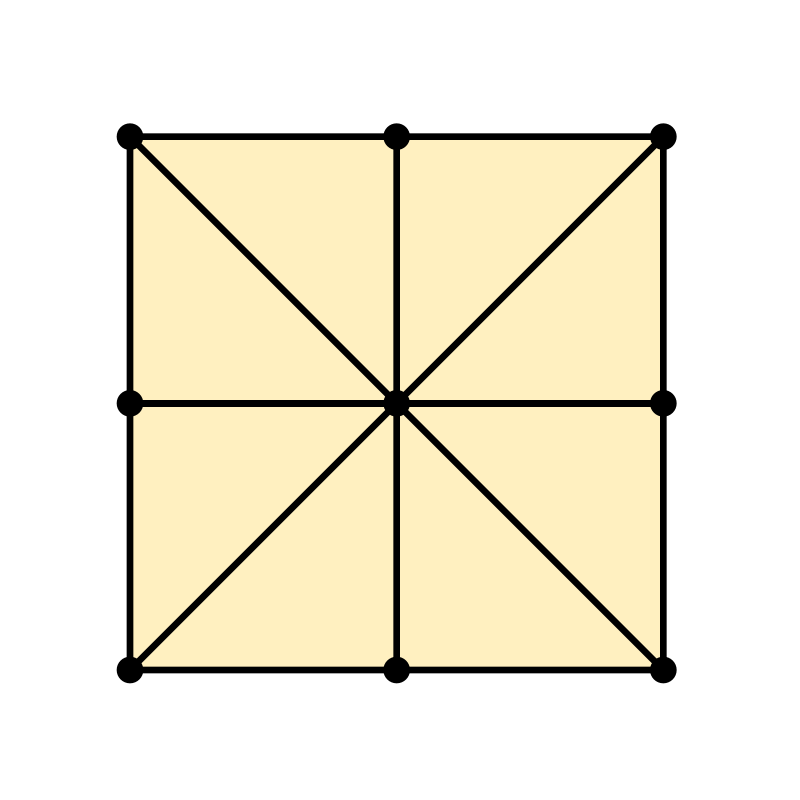
\includegraphics[width=4cm]{emptyboard.png}
    \caption{Empty three men's morris board \cite{wiki-image}}
    \label{fig:emptyboard}
  \end{center}
\end{figure}
